\section{Selected Confirmation Reconstructions}
\label{app:qualitative}
These examples are selected successes under the post-hoc rule in Section~\ref{sec:qualitative-summary}. They must be read with the complete cohort results, including regressions. The visualization pairs show original VGGT and the selected hypothesis. Table~\ref{tab:qualitative-cases} also reports the scalar comparison.

\begin{figure}[htbp]
\centering
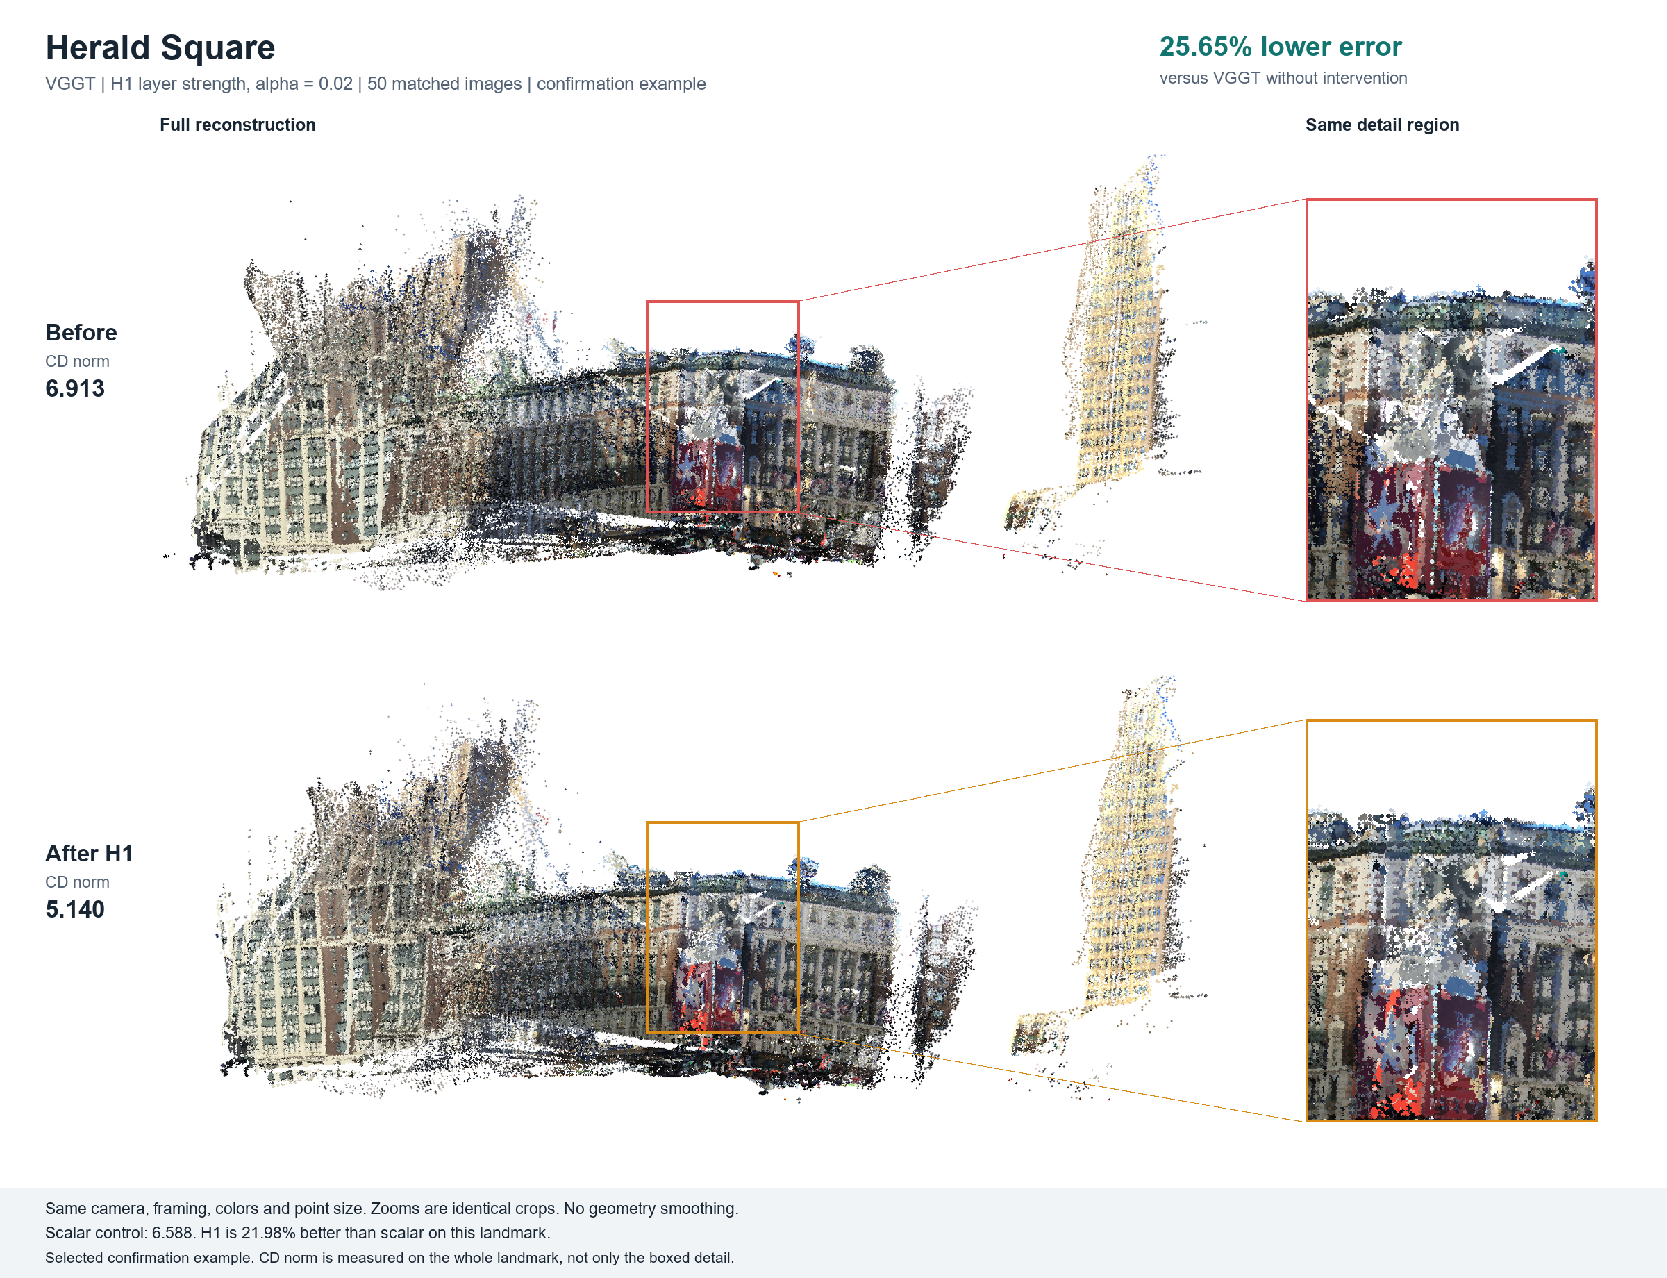
\includegraphics[width=\textwidth]{figures/qualitative_H1.pdf}
\caption{H1, Herald Square (facade). Whole-landmark error decreases by 25.65\% from original VGGT and 21.98\% from the scalar. The paired views share rendering and crop settings. The detail inset is not scored separately.}
\Description{Matched before and after point-cloud reconstructions of Herald Square with a common detail inset.}
\end{figure}
\clearpage
\begin{figure}[htbp]
\centering
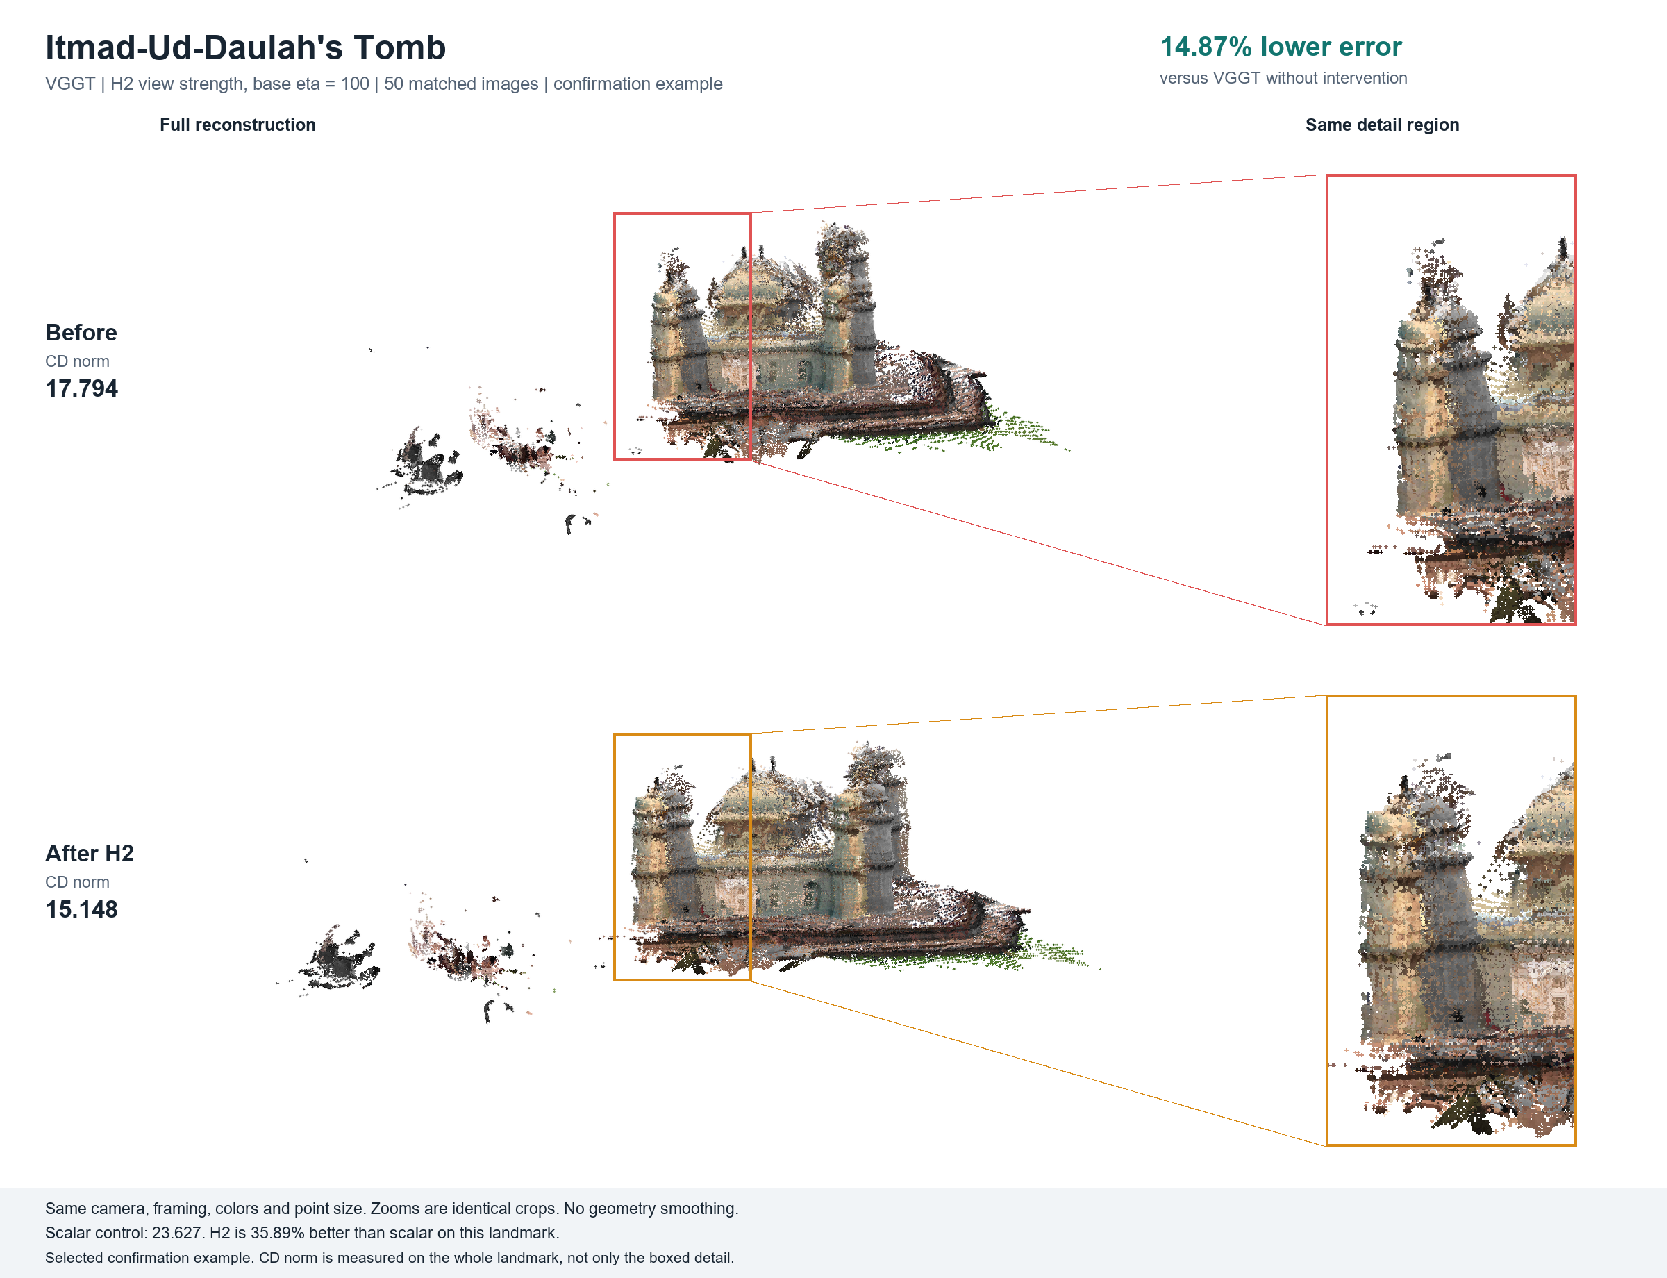
\includegraphics[width=\textwidth]{figures/qualitative_H2.pdf}
\caption{H2, Itmad-Ud-Daulah's Tomb (railing). Whole-landmark error decreases by 14.87\% from original VGGT and 35.89\% from the scalar. This selected success coexists with a worse cohort mean than original VGGT.}
\Description{Matched before and after point-cloud reconstructions of Itmad-Ud-Daulah's Tomb with a shared inset.}
\end{figure}
\clearpage
\begin{figure}[htbp]
\centering
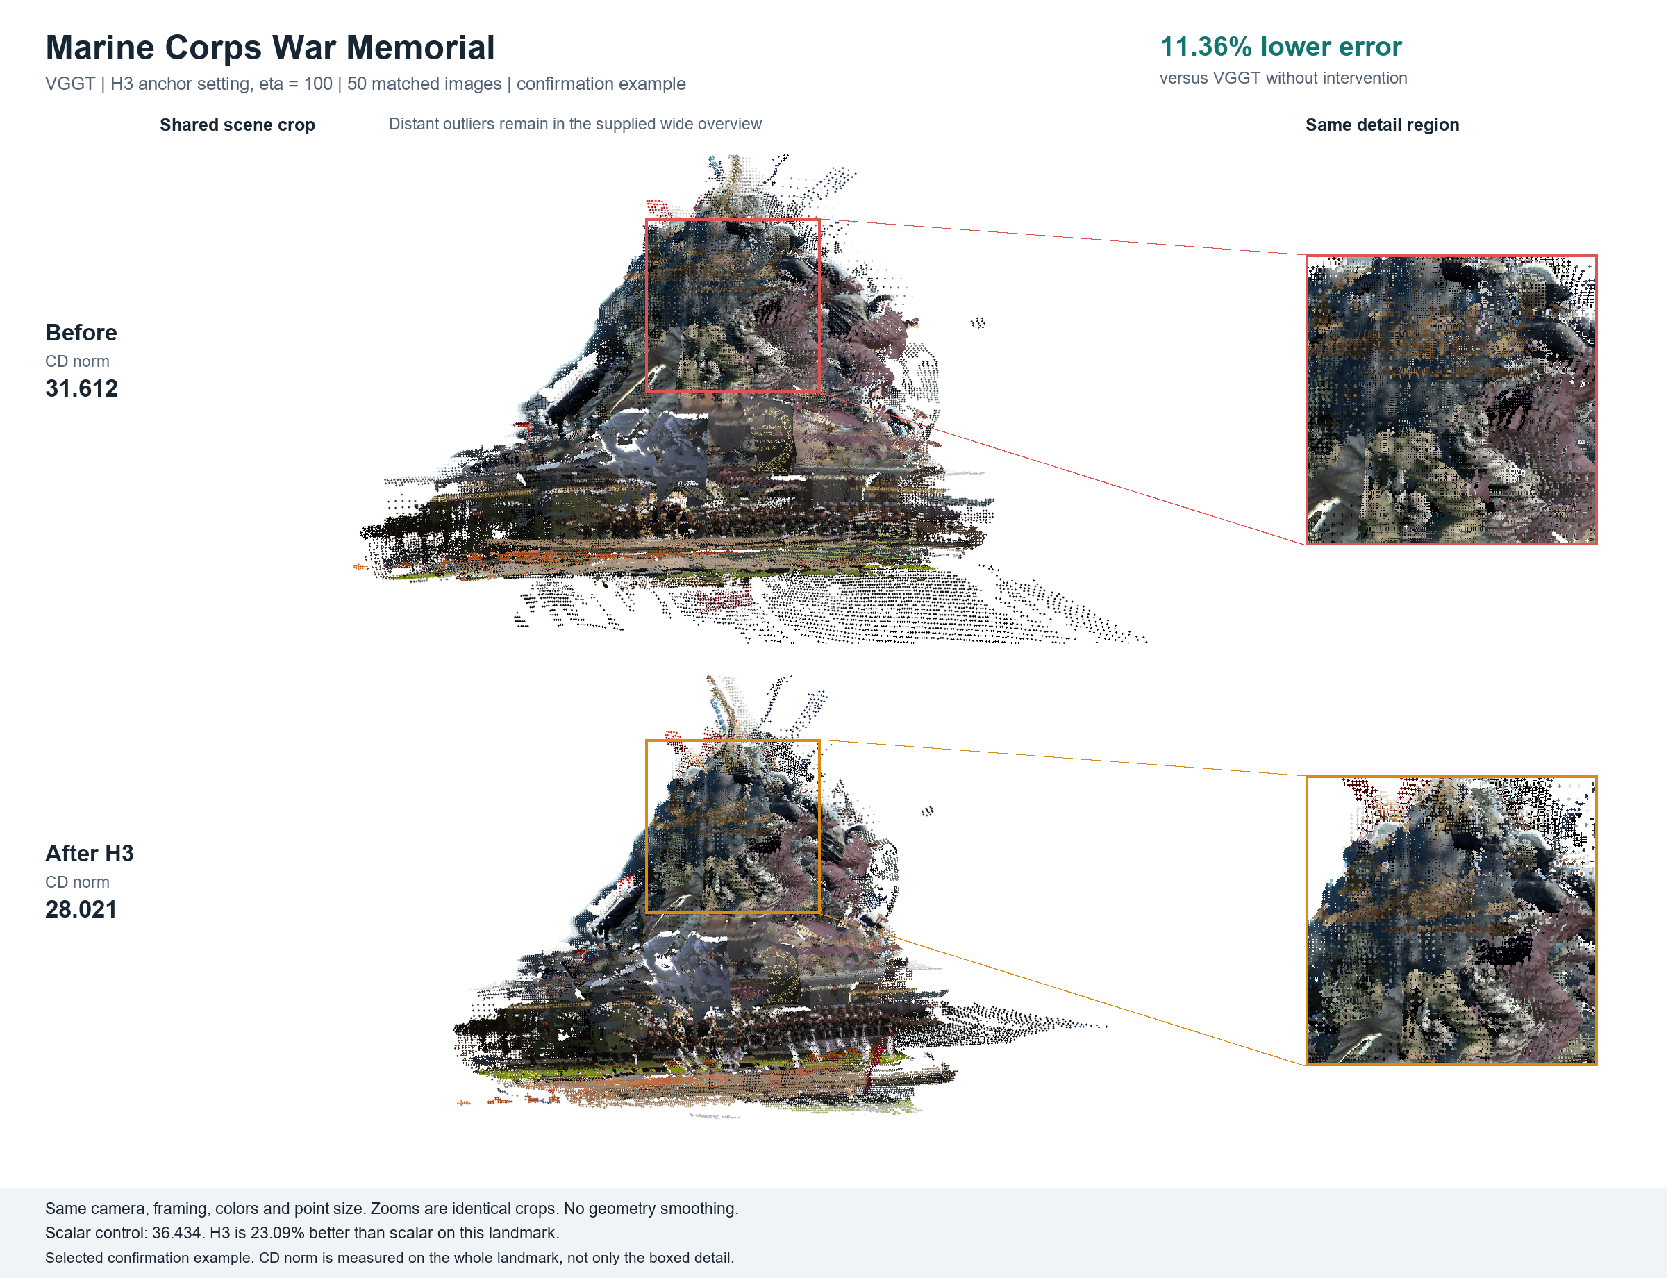
\includegraphics[width=\textwidth]{figures/qualitative_H3.pdf}
\caption{H3, Marine Corps War Memorial (statue). Whole-landmark error decreases by 11.36\% from original VGGT and 23.09\% from the scalar. A shared scene crop retains 99.13\% of original and 99.26\% of H3 points. The reported errors use the full evaluated clouds. The uncropped overview is supplied as \nolinkurl{figures/qualitative_H3_wide.pdf}.}
\Description{Original and H3 point-cloud renderings of Marine Corps War Memorial using the same scene crop and inset framing.}
\end{figure}
\clearpage
